\documentclass[a4paper]{article}
\usepackage{graphicx}
\usepackage{xcolor}
\usepackage{url}
\usepackage{outlines}
\usepackage{listings}
\usepackage{fontspec}
\lstset{basicstyle=\ttfamily,
	showstringspaces=false,
	commentstyle=\color{blue},
	keywordstyle=\color{pink}
}
\lstset{emph={
	EXPOSE,RUN,FROM,CMD,nc,tcp,udp,http,docker},emphstyle=\color{purple}
}
\usepackage{fancyhdr}
\usepackage{geometry}
\geometry{
	a4paper,
	total={170mm,257mm},
	left=20mm,
	top=20mm,
	bottom=39mm,
}

\setlength{\headheight}{82.70538pt}

\fancypagestyle{oida}{
	\fancyhf{}
	\fancyhead[L]{\fontsize{7.5}{7.5}htl donaustadt\\ Donaustadtstraße 45\\
		1220 Wien\\~\\ Abteilung: Informationstechnologie\\ 
	Schwerpunkt: Netzwerktechnik}
	\fancyhead[R]{
\includegraphics[scale=0.45]{images/logo.png}}

	\fancyfoot[L]{\today}
	\fancyfoot[C]{\jobname}
	\fancyfoot[R]{Page: \thepage}
}

\begin{document}
\bibliographystyle{plain}
\pagestyle{oida}
\section*{Thema}
\par\noindent\rule{\textwidth}{0.4pt}

Laboratory protocol
GNU/Linux - Setting up a multi-user environment

\begin{figure}[h]
	
\includegraphics[scale=0.3]{images/mika.jpeg}
	\caption{Grouplogo}
\end{figure}

\vspace*{\fill}
Subject:	ITSI|ZIVK

Class:	3AHITN

Name:	Stefan Fürst, Marcel Raichle

Groupname/number: Dumm und Dümmer/7

Supervisor: 	ZIVK

Exercise dates:	

Submission date:


\newpage
\tableofcontents

\newpage

\section{Task definition}



\section{Summary}


\newpage

\section{Exercise execution}

\subsection {creating the container}

I choose to write my own Dockerfile for this, which is a textfile, that describes the commands needed to create the desired image. Lets walkthrough how to create an image for the first task. \\
We start by using the \texttt{FROM} keyword to specify from the base image \cite{docker-glossary} from which we start.
\\
\texttt{FROM ubuntu:latest} \\
I choose the ubuntu image \cite{ubuntu} and used the \texttt{latest} tag, which points to the latest LTS release.\\
However if we were to build, start and exec into the container we wouldnt be able to do it beacouse it would imidiatly showdown, since nothing is running. \\

To midigate this we add \texttt{CMD tail -F /dev/null} at the end of out Dockerfile. The \texttt{tail} command outputs the last 10 lines of a file and the \texttt{-F} argument, which stands for follow so it runs forever outputting the last 10 lines of a given file.\cite{tail} I used file \texttt{/dev/null} which is a virtual device, that any data that gets written to vanishes. \cite{devnull} So we essentially read an empty file forever to keep the container up. \\

If we now run the following commands to build the image, run the container and get a shell in it.
\begin{lstlisting}[language=bash]
#build the image
docker buildx build -t image-name .
#run the container
docker run -d --name container-name 
#exec into the container (get a shell in it)
docker exec -it container-name /bin/bash
\end{lstlisting}
To make to commands less work to type, i like to make a shell script that i can source to have aliases for it like this.
\begin{lstlisting}[language=bash]
#!/bin/sh
alias relaunch="sudo sh -c 'docker stop itsi &&\
      docker rm itsi &&\
      docker buildx build -t itsi:latest . &&\
      docker run -d -p 38452:38452 --name itsi itsi:latest &&\
      docker exec -it itsi /bin/bash'"
alias rebuild="sudo sh -c 'docker buildx build -t itsi:latest . &&\
      docker run -d -p 38452:38452 --name itsi itsi:latest &&\
      docker exec -it itsi /bin/bash'"
alias stop="sudo sh -c 'docker stop itsi && docker rm itsi'"
\end{lstlisting}
Now we are in the container but it has none of the required Packages install that are required for this exercise. They can be installed now in the container which would defeat the entire purpose of making an image, so we use the \texttt{RUN} keyword in our Dockerfile along with the desired command to run it when the image is build so the packages are installed as soon as you spin up the container:
\begin{lstlisting}[language=bash]
RUN apt update 
RUN apt upgrade -y
RUN apt install iproute2 iputils-ping zsh net-tools vim -y
\end{lstlisting}
\newpage
\subsection{testing connectivity}
Now we can finally test the connectivity, since have the \texttt{iputils-ping} package installed. Everything works out of the box by using the default bridge \cite{Docker-bridge}

\begin{figure}[h]
	\centering
	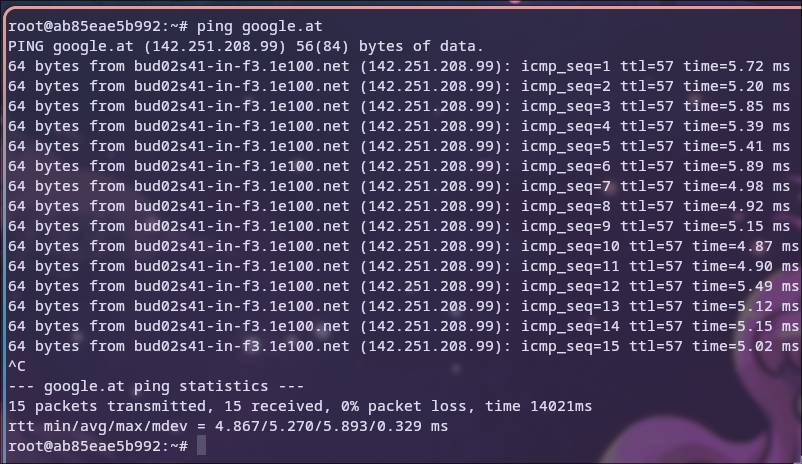
\includegraphics[scale=0.3]{images/ping_internet.png}
	\caption{ping to the internet}
\end{figure}
\begin{figure}[h]
	\centering
	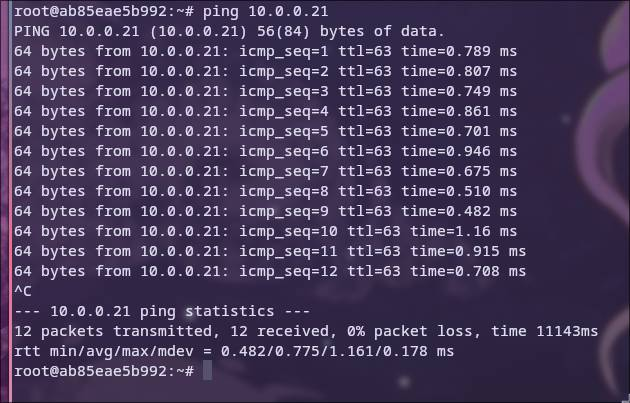
\includegraphics[scale=0.3]{images/ping_lokal.png}
	\caption{ping to the localnetwork}
\end{figure}
\newpage
\subsubsection {it works but why?}

If we inspect our container by using \texttt{docker inspect container-name}, we see that its ip is different than the ones from the lan.

\begin{figure}[h]
	\centering
	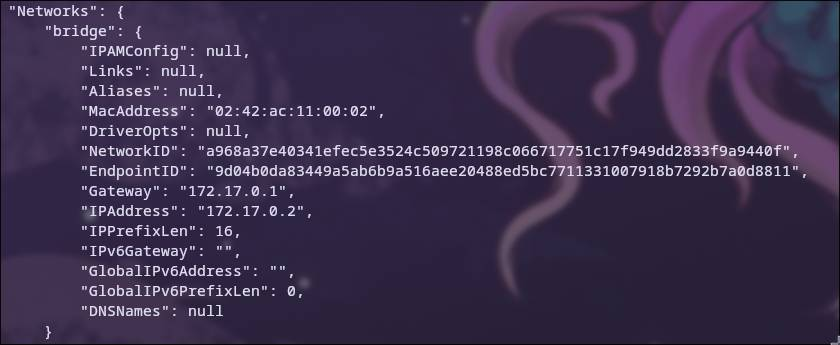
\includegraphics[scale=0.3]{images/docker_inspect_nw.png}
	\caption{docker inspect}
\end{figure}
This happens because when you install docker, a virtual interface \texttt{docker0} is created, which is used as a networkbridge to allow the container to communicate to the internet and lan. \cite{docker-networking-video}

\begin{figure}[h]
	\centering
	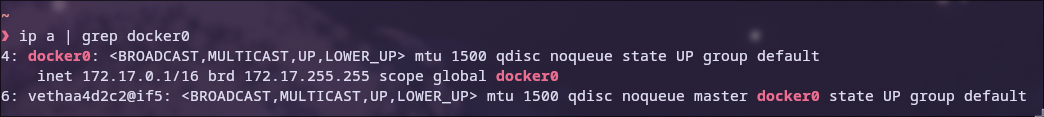
\includegraphics[scale=0.3]{images/ipadocker.png}
	\caption{ip a | grep docker0}
\end{figure}
There are other types of docker networks, but they arent relevant for this exercise.\cite{docker-networking-video}
\newpage
\subsection{creating and managing users}

For creating grous/users there are the commands \texttt{groupadd} and \texttt{useradd}.
To add the user we add the following lines to our Dockerfile
\begin{lstlisting}[language=bash]
#creating the group
RUN groupadd -g 324 ram-Users 
#creating the users -u is used to set the groupid
RUN useradd -u 1024 ram-alois &&\
    useradd -u 1124 ram-berta &&\
    useradd -u 1224 ram-chris &&\
    useradd ram-fus &&\
    useradd ram-ram
#adding the users to the groups
RUN usermod -g ram-Users ram-alois &&\
    usermod -g ram-Users ram-berta
#settings chris's default shell to zsh
RUN usermod --shell /bin/zsh ram-chris 
\end{lstlisting}
\subsubsection{logging in as the users}

To login as a different user the \texttt{su} command is used.

\begin{figure}[h]
	\centering
	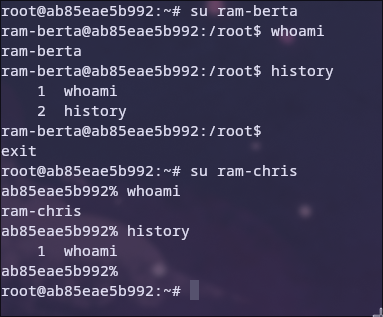
\includegraphics[scale=0.3]{images/logggingin.png}
	\caption{logging in as berta and chris}
\end{figure}
Each user has their own history, which is saved in their home directory in either the \texttt{.bash\_history} or \texttt{.zsh\_history} file. You end the session by using the \texttt{exit} command or pressing \texttt{<C-d>}.

\subsection {setting permissions for directories}
The directorys are created with this commad and the \texttt{-p} stands for parents and creates parent directorys if needed. For example \texttt{mkdir /test/test2} wouldn't work if you dont have \texttt{/test} but if you use \texttt{mkdir -p} instead it creates \texttt{/test} and \texttt{/test/test2}.

\begin{lstlisting}[language=bash]
RUN mkdir -p /data/fus &&\
    mkdir /data/fus/alois &&\
    mkdir /data/fus/berta &&\
    mkdir /data/fus/chris &&\
    mkdir /data/fus/public
\end{lstlisting}
To set the permission three tools will be used: \texttt{chrgrp}, \texttt{chown} and \texttt{chmod}. \\
First we want everyone in the group  to have acess to the directory for this \texttt{chgrp -R ram-Users /data/fus/} is used with the \texttt{-R} argument meaning recursive  \cite{perms,chgrp}
\\To give everyone every permission in their own directory, we need to make them the owner of it by using \texttt{chown -R username:groupname /data/fus/name-of-their-directory}.\cite{chown} \\
Now we can assign the permissions to each directory, for this the \texttt{chmod}\cite{chmod} command is used. \\
To better understand the command here is a breakdown of the options: \\ 
\begin{lstlisting}
u = user who owns the file
g = group -> everyone in the group of the owner
o = other -> everyone else
r = read
w = write
x = execute
+ adding permissions
- removing permissions
= setting permissions
\end{lstlisting} \cite{chmod}
Now lets use this to set the permissions accordingly
\begin{lstlisting}[language=bash]
#giving the [g]roup [r]ead and [w]write permissions for /data/fus
chmod g+rw /data/fus/
#giving the owner all permissions, the [g]roup only read [r]ead and none to [o]thers
chmod -R u+wrx,g=r,o= /data/fus/alois/
#same for berta
#giving the owner all permissions and none to the [g]roup and [o]thers
chmod -R u+wrx,g=,o= /data/fus/chris/ 
#giving the owner and [g]roup all permissions and none to [o]thers
chmod -R u+wrx,g+wrx,o=r /data/fus/public/
\end{lstlisting} \cite{chmod}
\begin{figure}[h]
	\centering
	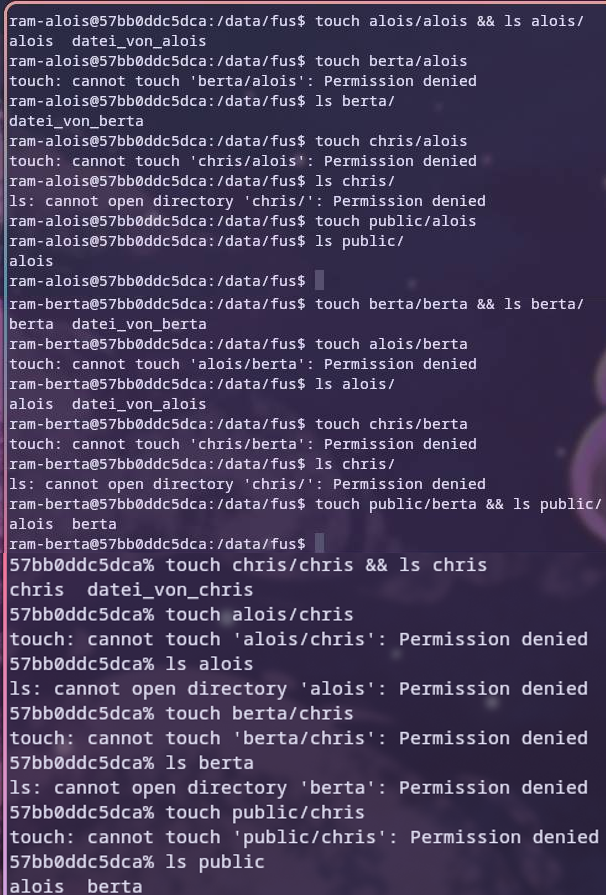
\includegraphics[scale=1.2]{images/testing_perms.png}
	\caption{testing the permissions}
\end{figure} \\
If we login as the users we can see that everything works as intended.
\newpage
\subsection {setting up ssh}
The two new users required for this have already been created above in 3.3 \\
To setup an ssh server we need to install the package if we just add \texttt{ssh} to our install command in the Dockefile we find out, that this commands requires interactions to set the timezone we need to add these two extra lines to the Dockerfile.
\begin{lstlisting}[language=bash]
#setting the timezone
RUN ln -fs /usr/share/zoneinfo/Europe/Vienna /etc/localtime
#running the command without it beeing interactive
RUN DEBIAN_FRONTEND=noninteractive apt install -y tzdata ssh
\end{lstlisting}
Now ssh is installed, but it needs to be started for this all we need to do is edit the last line of the file to launch the service aswell.
\begin{lstlisting}[language=bash]
#the default command from before
CMD tail -F /dev/null
#with starting ssh
CMD service ssh start && tail -F /dev/null
\end{lstlisting}
To find out on what port the server is listening for ssh we use the netstat command, which comes with the \texttt{net-tools} package, which we installed earlier.
For this the command \texttt{netstat -tunlp | grep ssh} is used. Here are the options of the command explained.
\begin{lstlisting}[language=bash]
-t show TCP ports
-u show UDP ports
-n show numerical addresses instead of resolving hosts
-l show only listening ports
-p show the PID of the listener's process
\end{lstlisting}\cite{netstat}
\begin{figure}[h]
	\centering
	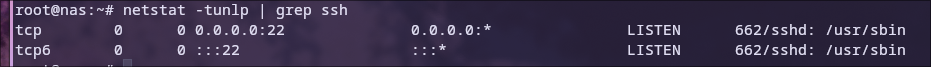
\includegraphics[scale=0.4]{images/netstatssh.png}
	\caption{finding the port with netstat}
\end{figure} \\
Appereantly its a "good practise" to move off the standart ssh port and use a different port to evade bots and script kiddies who are scanning the internet for public servers with ssh and testing default passwords. I belive that this is snake oil to change to port for better security, because if you disable password authentication, have a strong password or ban failing ips with tools such as fail2ban all of the problems are resolved anyway.\cite{hardening-linux-video} \\
I still changed to port to show how it would be done anyway.
For this we need to edit the file \texttt{/etc/ssh/sshd\_config}. \\
To do this we can use the preinstaleld texteditor \texttt{sed} so edit the file with the following command so we can change the port in the Dockerfile
\begin{lstlisting}[language=bash]
#-i edit the file in place without printing it to the console
#s to use the substitute command of sed
#'/s/string-you-want-to-replace/string-you-want-to-replace-it-with'
#/etc/ssh/sshd_config file that you want to edit
RUN sed -i 's/#Port 22/Port 38452/' /etc/ssh/sshd_config
\end{lstlisting}
If we try to ssh in with the created user we cant yet, since we havent published any ports in our container yet.
\subsubsection{logging into the ssh server}
\begin{figure}[h]
	\centering
	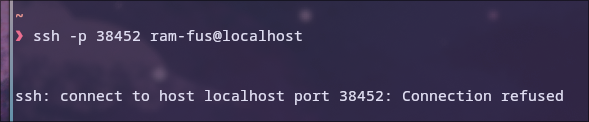
\includegraphics[scale=0.4]{images/loggingin-before-expsing-the-port.png}
	\caption{connection refused}
\end{figure} 
To do this we need to add one line to the Dockerfile and edit the docker run command.
\begin{lstlisting}[language=bash]
#add this to the with the port you choose to the Dockerfile
EXPOSE 38452
#add -p to [p]ublish the desired port
docker run -d -p 38452 --name container -name
\end{lstlisting}
Even if we login now it will still not work, since the user doens't have a password.
\begin{figure}[h]
	\centering
	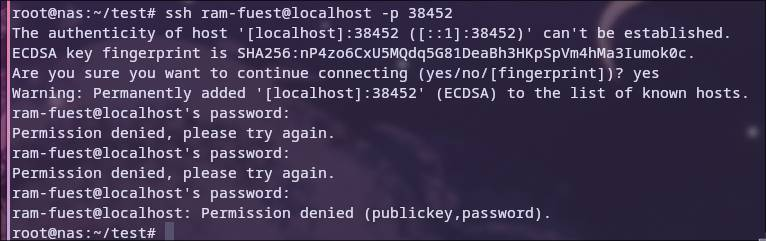
\includegraphics[scale=0.4]{images/failingtologin.png}
	\caption{logging without a password}
\end{figure} \\
To fix this we add this line to our Dockerfile:
\begin{lstlisting}[language=bash]
RUN echo 'root:youresecurepasswordhere' | chpasswd
\end{lstlisting}
We change the root password instead of the user password, since we dont have \texttt{sudo} setup and having to type sudo for every command, when we are the only user is both unecessary and anoing. 
\begin{figure}[h]
	\centering
	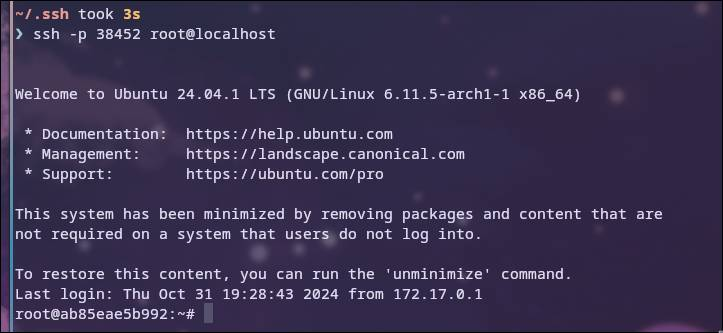
\includegraphics[scale=0.4]{images/workinglogin.png}
	\caption{working login}
\end{figure} \\
\newpage
\subsubsection{enabeling keypair authenthication}
To generate a keypair, we go back to out host system and run the comand \texttt{ssh-keygen -b 4096} to generate an 4096-bit SSH-Key. \cite{ssh-keygen}
On linux the keys get saved to the \texttt{~/.ssh} directory, but you can specify a location with \texttt{-f}. The file ending with \texttt{.pub} is the public key and the other one is the private key.
\begin{figure}[h]
	\centering
	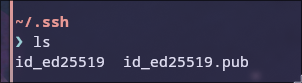
\includegraphics[scale=0.5]{images/keys-in-the-dir.png}
	\caption{keys in the directory}
\end{figure} \\
To copy the public key to the server, which we want to use it we the \texttt{ssh-copy-id} command on linux and \texttt{scp} on windows and mac. \cite{ssh-copy-id}
\begin{figure}[h]
	\centering
	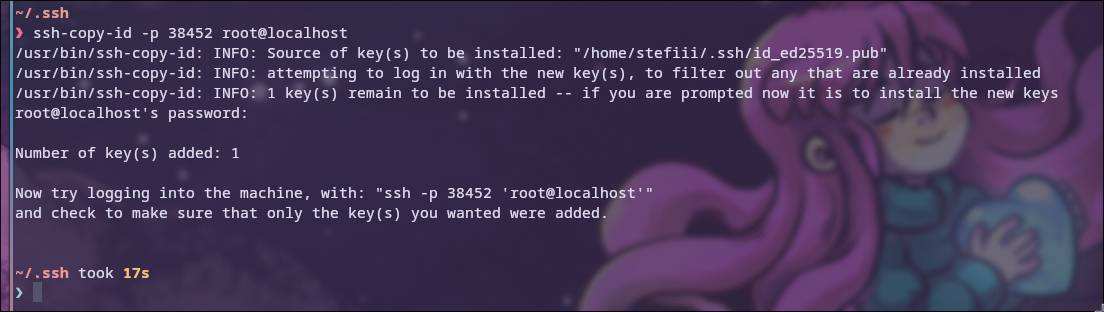
\includegraphics[scale=0.3]{images/ssh-copy-id.png}
	\caption{ssh-copy-id}
\end{figure} \\
After this if we dont need to enter a password anymore to authenticate.
\begin{figure}[h]
	\centering
	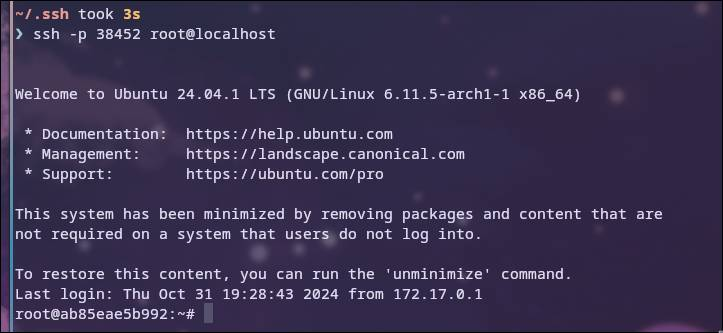
\includegraphics[scale=0.35]{images/login-with-key.png}
	\caption{logging with a key}
\end{figure} \\
\newpage
\subsubsection {disableling password authentication}
To only allow authetication via keys, we need to edit the file \texttt{/etc/ssh/sshd\_config} again.
To do this we ssh into the server and use open the file with the texteditor of your choice and edit this line.
\begin{lstlisting}[language=bash]
#change this
#PasswordAuthentication yes
#to this
PasswordAuthentication no
\end{lstlisting}
If we try to login as another user, for which we dont have a key we cant connect.
\begin{figure}[h]
	\centering
	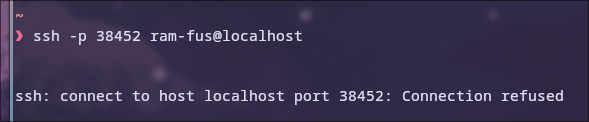
\includegraphics[scale=0.35]{images/nokey.png}
	\caption{not having a key}
\end{figure} \\
\newpage
\bibliography{quellen}
\newpage
\section{List of figures}

\listoffigures

\end{document}
